\section{Class 5 - 08/03/21}
\subsection*{characteristic impedance}
We can start this lecture by computing the derivative over the space of the voltage equation in phasor domain in \cref{eq:voltage_in_phas_domain}.
\begin{equation}
    \frac{\partial \phas{V}(z)}{\partial z}=\gamma \cdot \left(-V\bottomPlus\,e^{-\gamma z}+V\bottomMinus \,e^{\gamma z}\right) 
\end{equation}
Then from the first equation in \cref{eq:telegraph_in_phas_1} we can obtain another way to express the current in phasor domain:
\begin{equation}
    \phas{I}(z)=\overbrace{\frac{\gamma}{(R+j\omega L)}}^{\frac{1}{Z_0}}\left[V\bottomPlus \,e^{-\gamma z}-V\bottomMinus \,e^{\gamma z}\right]
\end{equation}
If we take a look on that equation, we can notice a very interesting pattern, that look like the ohm's law: $I=G\,V$ with $G$ the conductivity of the circuit, or the inverse of the resistivity.\\
If you look closely, also $\frac{\gamma}{(R+j\omega L)}$ is a conductance:
\begin{equation}
    \frac{\gamma}{(R+j\omega L)}=\frac{\sqrt{(R+j\omega L)\,(G+j\omega C)}}{(R+j\omega L)}=\sqrt{\frac{G+j\omega C}{R+j\omega L}}
\end{equation}
The inverse of that term is an impedance, and we call that \emph{characteristic impedance} (lol, what a fantasy):
\begin{equation}
    Z_0=\sqrt{\frac{R+j\omega L}{G+j\omega C}}\;\left[\Omega \right]
\end{equation}
Without losses, the same equation becomes:
\begin{equation} \label{eq:characteristic_impedance_no_loss}
    Z_0=\sqrt{\frac{j\omega L}{j\omega C}}=\sqrt{\frac{L}{C}}
\end{equation}
If you look closely, \cref{eq:characteristic_impedance_no_loss} is very similar to the intrinsic impedance $\eta = \sqrt{\frac{\mu}{\varepsilon}}$ (\cref{eq:intrinsic_impedance}).\\
The current and current expression becomes:
\begin{equation}
    \begin{cases}
    \phas{V}(z) = V\bottomPlus \,e^{-j\beta z}+V\bottomMinus \,e^{j\beta z} \\[5pt]
    \phas{I}(z)=\frac{1}{Z_0}\left[V\bottomPlus \,e^{-\gamma z}-V\bottomMinus \,e^{\gamma z}\right]
    \end{cases}\label{eq:current_and_voltage_in_TL_phas}
\end{equation}
From now on, sometimes I could miss some phasor notation over $V$ and $I$, this was very important to emphasize the difference between the different domains, but no the next pages if you see $V(l)$ or $I(l)$ just remember that those wave expression does not contain the time $t$, so they are in phasor domain.\\
That being said, we can also write:
\begin{align}
    \begin{split}
      &V\bottomMinus = - Z_0 \,I\bottomMinus \\[5pt]
      &V\bottomPlus = Z_0 \,I\bottomPlus 
    \end{split}
\end{align}

\subsection*{Input impedance}
\begin{figure}[H]
    \begin{center}
        \begin{circuitikz} [ baseline=(current bounding box.center)]
            \ctikzset { label/align = straight }
            \draw (0,3)
            node[label={[font=\normalsize]above:$in$}] {}
            to[short, o-o,] (7,3)
            node[label={[font=\normalsize]above:$out$}] {}
            to[short](8.5,3)
            to[generic=$Z_{l}$] (8.5,0)
            to[short](7,0)
            to[short, o-o,] (0,0)
            ;
            \draw [-|] (0,-0.5) -- (7,-0.5)
            node[label={[font=\large]below:$0$}] {}
            ;
            \draw [->] (7,-0.5) -- (9,-0.5)
            node[label={[font=\large]right:$l$}] {}
            ;
            \draw (4,1)node[label={[font=\LARGE]above:$Z_0$}] {}
            ;
          \end{circuitikz}     
    \end{center} \caption{Transmission line with reference system}\label{fig:general_transmission_line_ref}
  \end{figure}
We assume that our transmission line is like in \cref{fig:general_transmission_line_ref}, here you can see that we introduced a reference system on the length of the line. The new coordinate $l$ is increasing on the right, and the zero point is set on the output coordinate of the line.
Starting from the equation of the signal over the line (with no losses) in \cref{eq:wave_solution_no_losses}, we can obtain the \emph{input impedance} of the line dependent on the position $l$:
\begin{align}
    \begin{split}\label{eq:input_impedance}
      Z_i(l)&=\frac{\phas{V}(l)}{\phas{I}(l)}=\frac{V\bottomPlus \,e^{-j\beta z}+V\bottomMinus \,e^{j\beta z}}{I\bottomPlus \,e^{-j\beta z}+I\bottomMinus \,e^{j\beta z}}\\[5pt]
      &=Z_0\,\frac{V\bottomPlus \,e^{-j\beta z}+V\bottomMinus \,e^{j\beta z}}{V\bottomPlus \,e^{-j\beta z}-V\bottomMinus \,e^{j\beta z}}
    \end{split}
\end{align}
Note that $Z_i(l)$ and $Z_0$ are very different, the first one can depend on the position over the line. But we can notice an important relation between the two when we are in $l=0$:
\begin{equation}\label{eq:input_impedance_l=0}
    Z_i(l=0)=Z_L=\frac{V_L}{I_L}=Z_0 \,\frac{V\bottomPlus +V\bottomMinus }{V\bottomPlus -V\bottomMinus }
\end{equation}
\subsubsection*{To not make confusion!}
All this notation is very confusing in my opinion, so a fast clarification:
\begin{itemize}
    \item $Z_0$ is the characteristic impedance, it is the same for all the line and can be considered like the impedance of the tiny tiny section of the TL.
    \item $Z_i(l)$ is the impedance that you would measure if you take a very special oscilloscope in a specific position $l$ on your line.\\
    If you are in $l=0$ you are measuring the load ($Z_L$).\\
    If you are in $l=L$ you are measuring the impedance on the input side of the TL (also named input impedance), so what impedance your generator see ($Z_{in}$).
    \item $\phas{V}(l)$ is the voltage that you would measure if you take a special oscilloscope in a specific position $l$ on your line (in phasor domain).
    \item $V_L$ is the voltage that the load see, that is also $\phas{V}(0)$.
    \item $V\bottomPlus$ is the progressive component of the voltage over the line, think at it like the module of the progressive voltage wave. It is a part of the wave equation solution. 
    \item $\phas{V_p}(z)=V\bottomPlus \,e^{-j\beta z}$ is the progressive (or incident) voltage wave equation over the line in phasor domain.
    \item $v(z,t)$ is the real voltage over the line and over the time, we are not using it because it is very difficult to manipulate, so we prefer to go in complex domain, then going back to time domain with simpler calculations
\end{itemize}
Still very confusing, I know (\textgreater\_\textless).
\subsubsection*{Input impedance in trigonometric form}
As we can see from the final form of the input impedance of \cref{eq:input_impedance}, $Z_i$ is a complex number, so it could be useful to express it in trigonometric form (you should remember $a\,e^{j\,b}=a(\cos\,b+j\sin\,b)$ ).\\
Now the calculation can seems scary, but they are very simple but long:
\begin{align}
    \begin{split}
      Z_i(l)&=Z_0\,\frac{V\bottomPlus \,e^{-j\beta l}+V\bottomMinus \,e^{j\beta l}}{V\bottomPlus \,e^{-j\beta l}-V\bottomMinus \,e^{j\beta l}}=\\[5pt]
      &=Z_0\frac{V\bottomPlus [\cos(\beta\, l)-j \, \sin(\beta\, l)]+V\bottomMinus [\cos(\beta\, l)+j \, \sin(\beta\, l)]}{V\bottomPlus [\cos(\beta\, l)-j \, \sin(\beta\, l)]-V\bottomMinus [\cos(\beta\, l)+j \, \sin(\beta\, l)]}=\\[5pt]
      &=Z_0\,\frac{(V\bottomPlus +V\bottomMinus )\,\cos(\beta\,l)-j(V\bottomPlus -V\bottomMinus )\,\sin(\beta\, l)}{(V\bottomPlus -V\bottomMinus )\,\cos(\beta\,l)-j(V\bottomPlus +V\bottomMinus )\,\sin(\beta\, l)}\cdot \frac{\frac{1}{(V\bottomPlus-V\bottomMinus)}}{\frac{1}{(V\bottomPlus-V\bottomMinus)}}=\\[5pt]
      &=Z_0\frac{\frac{Z_L}{Z_0}\cos(\beta\,l)-j\,\sin(\beta \,l)}{\cos(\beta\, l)-j\,\frac{Z_L}{Z_0}\sin(\beta l)}=\\[5pt]
      &=Z_0\frac{Z_L\,\cos(\beta \,l)-j\,Z_0\,\sin(\beta \, l)}{Z_0\, \cos(\beta \, l)-j\,Z_L\,\sin(\beta \, l)}
    \end{split}
\end{align}
Now for the sake of simplicity we say that $l$ is not the coordinate of the point where we are looking over the line, but the distance from the $0$ point.\\
In this case, the $Z_i(l)$ equation of the input impedance becomes a bit simpler (it only changes a couple of sign):
\begin{equation}\label{eq:input_impedance_1}
    Z_i(l)=Z_0\frac{Z_L\,\cos(\beta \,l)+j\,Z_0\,\sin(\beta \, l)}{Z_0\, \cos(\beta \, l)+j\,Z_L\,\sin(\beta \, l)}
\end{equation}
In terms of admittance, the \cref{eq:input_impedance_1} becomes:
\begin{equation}
    Y_i(l)=Y_0\frac{Y_L\,\cos(\beta \,l)+j\,Y_0\,\sin(\beta \, l)}{Y_0\, \cos(\beta \, l)+j\,Y_L\,\sin(\beta \, l)}
\end{equation}
\subsection*{Reflection coefficient}
\begin{figure}[H]
    \begin{center}
        \begin{circuitikz} [%
            wave/.style={%
              ->,
              shorten >=4pt,
              shorten <=4pt,
              decorate,
              decoration={%
                snake,
                segment length=3mm,
                amplitude=0.4mm,
                pre length=4pt,
                post length=4pt,
              }
            }
          ]
            \draw (0,0)
            to[sV=$V_{g}$] (0,2.5)
            to[R=$R_{g}$, -o] (2,2.5)
            to[short, -o] (7,2.5)
            to[short] (8.5,2.5)
            to[generic=$Z_{l}$] (8.5,0)
            to[short, -o](7,0)
            to[short, -o](2,0)
            to[short](0,0)
            ;
            \draw [wave] (2,2.2) -- (7,2.2)
            node[midway,yshift=-1em]{$V_p$}
            ;
            \draw [wave] (7,0.3) -- (2,0.3)
            node[midway,yshift=1em]{$V_r$}
            ;
          \end{circuitikz}     
    \end{center} \caption{Forward and backward wave signal in a TL}\label{fig:forward_and_backward_wave} 
\end{figure}
In \cref{fig:forward_and_backward_wave} you can see a very common example of how the signal propagates in a TL when a load $Z_l$ is connected: we have both a forward and backward wave inside the same medium (ex. coaxial cable).\\
The forward signal $V\bottomPlus$ is the one that we like, the backward $V\bottomMinus$ is not helpful for us, and it cause unwanted interference (by adding to the forward one, and making a mess).\\
To describe a bit better this situation, we can introduce the \emph{reflection coefficient} $\rho(l)$, that define the reflected wave with respect to the incident wave:
\begin{equation}\label{eq:definition_of_rho}
    \rho(l) = \frac{V\bottomMinus\,e^{-j\,\beta\,l}}{V\bottomPlus\,e^{\,j\,\beta\,l}}=\frac{V\bottomMinus}{V\bottomPlus}\,e^{\,-j2\beta l}
\end{equation}
\begin{equation}\label{eq:definition_of_rho2}
    \rho(l) = \frac{Z_i(l)-Z_0}{Z_i(l)+Z_0}
\end{equation}
Note that the amplitude of $\rho(l)$ is always fixed along $l$, and only the exponential part $e^{\,j2\beta l}$ is dependent on $l$ (I don't really know why this is important \dunno).\\
Keep in mind that this reflection coefficient relates on the position over the line.
\subsubsection*{Reflection coefficient at the load}
If you place a load $Z_L$ at the output of the transmission line, and you measure the voltage $V(l=0)$ and the current $I(l=0)$ at the end of that TL ($l=0$), you can have the \emph{reflection coefficient at the load} $\rho_L$:
\begin{equation}\label{eq:reflection_coeff_at_load}
    \rho(l=0)=\rho_L=\frac{V\bottomMinus}{V\bottomPlus}=\frac{Z_L-Z_0}{Z_L+Z_0}
\end{equation}
From \cref{eq:definition_of_rho} we can write:
\begin{equation}\label{eq:reflection_coeff_at_load2}
    \rho(l)=\rho_L\,e^{\,j2\beta l}
\end{equation}
This is a parameter that is used to define the reflected wave with respect to the
incident wave on the load, and I think that it is much more easy to understand than $\rho(l)$.
If you look closely at \cref{eq:reflection_coeff_at_load}, it is possible to have $\rho_L=0$ when $Z_L=Z_0$. The explanation that the prof gave to us is a little confusing for me, but it works like the wave is always seeing $Z_0$ while it is travelling along all the tiny portion of TL; when the wave arrives to $Z_L$, it sees no difference, so for him it is like the TL is infinite.\\
Note that sometimes the reflection coefficient $\rho_L$ is written like only the symbol $\rho$. This is a little confusing, but it simplify a lot the notation.
\subsubsection*{Little exercise!}
We have a transmission line with:
\begin{itemize}
    \item characteristic impedance $Z_0 = 100 \si{\ohm}$
    \item Load resistance $R_L=50 \si{\ohm}$ 
    \item Load capacitance $C_L=10 \si{\pico\farad}$
    \item Frequency of the generator $f=100\si{\mega\hertz}$
\end{itemize}
The question is: \textbf{What is the value of $\rho(l)$ and $\rho_L$?}
First of all we can calculate the load impedance in phasor domain $Z_l$
\begin{equation*}
    Z_l=R_L+\frac{1}{j\omega C_L}=R_L-j\,\frac{1}{\omega C_L}=\cdots =50-j\,159\;\Omega
\end{equation*}
Then it is simple to obtain $\rho_L$:
\begin{equation*}
    \rho_L =\frac{Z_L-Z_0}{Z_L+Z_0}=\cdots =-0.76\,e^{\,j119^{\circ}}
\end{equation*}
In this case the 76\% of the signal is reflected back to the emitter, very bad! :(\\
now let's calculate $\rho(l)$:
\begin{equation*}
    \rho(l)=\rho_L\,e^{\,j2\beta l}=\rho_L\,e^{\,j2\frac{\omega}{c} l}=-0.76\,e^{\,j119^{\circ}}\,e^{\,j 2\pi 33.3 l}
\end{equation*}
\subsubsection*{Normalized impedance and reflection coefficient}
Sometimes it could be useful to use \emph{normalized input impedance}:
\begin{equation}
    \mathcal{Z}_i =\frac{Z_i}{Z_0}
\end{equation}
And also the \emph{normalized load impedance}
\begin{equation}
    \mathcal{Z}_L =\frac{Z_L}{Z_0}
\end{equation}
Then the reflection coefficient becomes:
\begin{center}
    \begin{tabular}{ c c c }
        $\rho(l)=\frac{\mathcal{Z}_i(l)-1}{\mathcal{Z}_i(l)+1}$&
        and&
        $\rho_L=\frac{\mathcal{Z}_L-1}{\mathcal{Z}_L+1}$
    \end{tabular}
\end{center}
\subsection*{Transmission line wth a short circuit}
\begin{figure}[H]
    \begin{center}
        \begin{circuitikz} [ baseline=(current bounding box.center)]
            \ctikzset { label/align = straight }
            \draw (0,3)
            node[label={[font=\normalsize]above:$in$}] {}
            to[short, o-o,] (7,3)
            node[label={[font=\normalsize]above:$out$}] {}
            to[short](8.5,3)
            to[short={$Z_{l}=0$}] (8.5,0)
            to[short](7,0)
            to[short, o-o,] (0,0)
            ;
            \draw [-|] (0,-0.5) -- (7,-0.5)
            node[label={[font=\large]below:$0$}] {}
            ;
            \draw [->] (7,-0.5) -- (9,-0.5)
            node[label={[font=\large]right:$l$}] {}
            ;
            \draw (4,1)node[label={[font=\LARGE]above:$Z_0$}] {}
            ;
          \end{circuitikz}     
    \end{center} \caption{Transmission line with short circuit load}\label{fig:transmission_line_short}
  \end{figure}
If we put a short circuit in the load side as in \cref{fig:transmission_line_short}, we can notice some useful property.\\
First of all we know that the voltage on the load is $0\si{\volt}$, so:
\begin{equation}
    V(l=0)=V_L=0=V\bottomPlus+V\bottomMinus \;\rightarrow \;V\bottomPlus=-V\bottomMinus
\end{equation}
This mean that the the reflection coefficient at the load is:
\begin{equation}
    \rho_L=\frac{V\bottomMinus}{V\bottomPlus}=\frac{-V\bottomPlus}{V\bottomPlus}=-1
\end{equation}
This means that:
\begin{center}
    \begin{tabular}{ c c c }
        $|\rho_L|=1$&
        and&
        $\phase{\rho_L}=180^{\circ}$
    \end{tabular}
\end{center}
In other words, if you place a short circuit as load of your TL, the incident wave will be 100\% reflected and it will also be shifted by $\pi$ (\cref{fig:signal_with_Z_0})
\begin{figure}[H]
    \begin{center}
        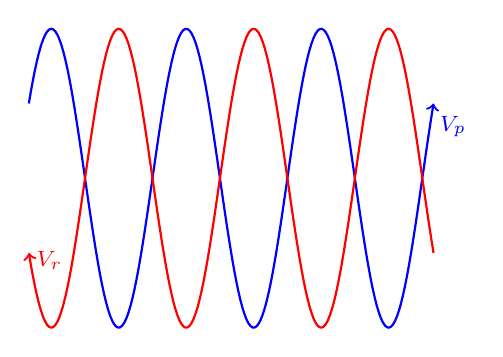
\begin{tikzpicture}
            \begin{axis}[
            axis x line=none,
            axis y line=none,
            ymax=1.5,
            ymin=-1.5,
            xmin=-pi,xmax=(pi*6)+(pi),
            x label style={anchor=north},,
            yticklabels={,,},
            xticklabels={,,},
            xtick=\empty,
            ytick=\empty,
            ]
            \addplot[domain=0:6*pi,samples=200,blue,thick,->]{cos(deg(x-pi/3))}
            node[right,pos=.99,font=\footnotesize]{$V_p$};
            \addplot[domain=0:6*pi,samples=200,red,thick,<-]{cos(deg(x-pi*1/3+pi))}
            node[left,pos=.1,font=\footnotesize]{$V_r$};
            \end{axis}
        \end{tikzpicture}        
    \end{center}
    \caption{Incident and reflected signal when $Z_L=0$}\label{fig:signal_with_Z_0}
\end{figure}
The voltage and the current over the line is:
\begin{equation}
    \begin{cases}
      V(l)&=V\bottomPlus\,e^{\,-j\beta l}-V\bottomMinus\,e^{\,j\beta l}=V\bottomPlus(e^{\,-j\beta l}+e^{\,j\beta l})=-2\,jV\bottomPlus\sin (\beta l)\\[5pt]
      I(l)&=\frac{V\bottomPlus}{Z_0}e^{\,-j\beta l}+\frac{V\bottomPlus}{Z_0}e^{\,j\beta l}=2\frac{V\bottomPlus}{Z_0}\cos (\beta l)
    \end{cases}
\end{equation}
So knowing only that $V\bottomPlus=-V\bottomMinus$ we can derive the voltage and current wave.\\
$\bullet$ If we go back in time domain:
\begin{align}
    \begin{split}
      V(l,t)&=\operatorname{Re}\left\{V(l)\,e^{\,j\omega t}\right\}=\operatorname{Re}\left\{j 2V\bottomPlus\sin (\beta l)\,e^{\,j\omega t}\right\}=\\[5pt]
      &=\operatorname{Re}\left\{j2V\bottomPlus\sin(\beta l)\,(\cos(\omega t)+j\sin(\omega t))\right\}=\\[5pt]
      &=-2\,|V\bottomPlus|\,\sin(\beta l)\sin(\omega t)
    \end{split}
\end{align}
Note that this is the equation of a \emph{stationary wave}! this mean that the voltage is moving across the line, but no information is transmitted from te generator to the load.\\
We can identify the stationary wave when $\beta l$ and $\omega t$ are in different $\cos$ (or $\sin$) operator.\\
$\bullet$ Power of this stationary wave:
\begin{align}
    \begin{split}
      P&=\frac{1}{2}V\cdot I^{*}=\frac{1}{2}\,\left(-2jV\bottomPlus \sin(\beta l)\right)\,\left(2\frac{V\bottomPlus}{Z_0}\cos(\beta l)\right)^*\\[5pt]
      &=-j2\frac{|V\bottomPlus|^2}{Z_0}\sin(\beta l)\cos(\beta l)
    \end{split}
\end{align}
Notice that the power is completely imaginary, this mean that we are transmitting only reactive power.\\
$\bullet$ The input impedance:
\begin{equation}\label{input_impedance_of_a_short}
    Z_i(l)=Z_0\frac{\cancelto{0}{Z_L}\cos(\beta l)+jZ_0 \sin(\beta l)}{Z_0\cos(\beta l)+j\cancelto{0}{Z_L}\sin(\beta l)}=jZ_0\tan(\beta l)
\end{equation}
$\bullet$ The input admittance:
\begin{equation}\label{input_admittance_of_an_open}
    Y_i(l)=\frac{1}{Z_i(l)}=\frac{1}{jZ_0\tan(\beta l)}=-Y_0\cot(\beta l)
\end{equation}
We again see that this input impedance is completely imaginary, so could be seen by the input port as a capacitor or an inductor depending on the sign of this imaginary number.\\
If we plot the behavior of $Z_i$ over $\frac{l}{\lambda}$ we have a graphical way to see this behavior (\cref{fig:behavior_of_short_in_TL}):
\begin{figure}[H]
    \begin{center}
        \begin{tikzpicture}
            \begin{axis}[
                axis x line=middle,
                axis y line=middle,
                xmin=-1.1,xmax=0.15,ymin=-4.5,ymax=4.5,
                x label style={anchor=north},
                xlabel= $\frac{l}{\lambda}$,
                ylabel={$Z_i$},
                yticklabels={,,},
                ytick=\empty,
                xticklabels={-1,-0.75,...,0},
                xtick={-1,-0.75,...,0},
                ]
              \addplot[domain=-1.1:0,blue,samples=200] {tan(deg(-x*2*3.14159))};
              \draw[dashed,red] (-1,-5) -- (-1,5);
              \draw[dashed,red] (-0.5,-5) -- (-0.5,5);

              \par\ctikzset{bipoles/capacitor/width=.1,bipoles/capacitor/height=.25}
              \draw (-0.9,-2.5) to [C] (-0.9,-1.5);
              \draw (-0.4,-2.5) to [C] (-0.4,-1.5);

              \par\ctikzset{bipoles/cuteinductor/width=.2,bipoles/cuteinductor/height=.25,bipoles/cuteinductor/coils=3}
              \draw (-0.6,2.5) to [cute inductor] (-0.6,1.5);
              \draw (-0.1,2.5) to [cute inductor] (-0.1,1.5);
              \draw (-1.07,2.5) to [cute inductor] (-1.07,1.5);
            \end{axis}
            
            \end{tikzpicture}       
    \end{center}
    \caption{Behavior of $Z_i$ a TL if the load is a short}\label{fig:behavior_of_short_in_TL}
\end{figure}
\subsubsection*{Another little exercise}
We have the usual information of our TL, but we know that the load is a short and on the behavior of the line is inductive; we need to find the length of the TL in order to have that behavior.\\
Data:
\begin{itemize}
    \item $v_p=2.07\cdot 10^{8}\si{\metre \per \second}$ speed of the signal.
    \item $L=15\si{\nano\henry}$ behavior of the TL.
    \item $f=3\si{\giga\hertz}$ frequency of the signal.
    \item $Z_0=50\si{\ohm}$ characteristic impedance of the TL.
\end{itemize}
Find length $l$.\\
$\bullet$ First of all we know that the load is a short, so:
\begin{equation*}
    Z_i(l)=jZ_0\, \tan(\beta l)
\end{equation*}
We also know that:
\begin{equation*}
    Z_i(l)=j\omega L
\end{equation*}
We go on to find the value of $l$:
\begin{align*}
    \begin{split}
      &Z_0\,\tan(\beta l)=\omega l\\[5pt]
      &\beta l=\arctan(\frac{\omega l}{Z_0})\\[5pt]
      &l=\frac{\lambda}{2\pi}\,\arctan(\frac{\omega l}{Z_0})=1.53\si{\centi\metre}
    \end{split}
\end{align*}
This mean that if my TL described by the data I gave before measure $1.53\si{\centi\metre}$, at the eye of the transmitter the TL is an inductor of $L=15\si{\nano\henry}$.\\
$\bullet$ If we change $f=4\si{\giga\hertz}$? Nothing to worry about:
\begin{equation*}
    \frac{l}{\lambda}=\frac{l\cdot f}{v_p}=0.3\geq 0.25
\end{equation*}
Assuming that \cref{fig:behavior_of_short_in_TL} is right, now the circuit should behave like a capacitor
Then we calculate $Z_i$:
\begin{equation*}
    Z_i=jZ_0\tan(\beta l)=jZ_0\tan(\frac{\omega}{v_p} l)=-j167.4
\end{equation*}
We obtained a negative imaginary impedance, so this is a capacitor!
\begin{equation*}
    -j\frac{1}{\omega C}=-j167.4 \rightarrow C=0.238\si{\pico\farad}
\end{equation*}
\subsection*{Transmission line wth an open circuit}
\begin{figure}[H]
    \begin{center}
        \begin{circuitikz} [ baseline=(current bounding box.center)]
            \ctikzset { label/align = straight }
            \draw (0,3)
            node[label={[font=\normalsize]above:$in$}] {}
            to[short, o-o,] (7,3)
            node[label={[font=\normalsize]above:$out$}] {}
            to[open](7.4,3)
            to[open={$Z_{l}=\infty$}] (7.4,0)
            to[open](7,0)
            to[short, o-o,] (0,0)
            ;
            \draw [-|] (0,-0.5) -- (7,-0.5)
            node[label={[font=\large]below:$0$}] {}
            ;
            \draw [->] (7,-0.5) -- (7.8,-0.5)
            node[label={[font=\large]right:$l$}] {}
            ;
            \draw (4,1)node[label={[font=\LARGE]above:$Z_0$}] {}
            ;
          \end{circuitikz}     
    \end{center} \caption{Transmission line with open circuit load}\label{fig:transmission_line_open}
  \end{figure}
In this case we do the opposite as before, we put an open circuit at the output of the TL, in this case $Z_L=\infty$.\\
Instead to have the voltage equal to 0 at the load, we have the current equal to zero:
\begin{equation}
    I(l)=\frac{V\bottomPlus}{Z_0}\,e^{\,-j\omega l}-\frac{V\bottomMinus}{Z_0}\,e^{\,j\omega l}
\end{equation}
\begin{equation}
    I(l=0)=I_L=0=I\bottomPlus+I\bottomMinus = \frac{1}{Z_0}\,\left[V\bottomPlus-V\bottomMinus\right] \;\rightarrow \;V\bottomPlus=V\bottomMinus
\end{equation}
$\bullet$ For the reflection coefficient this mean:
\begin{equation}
    \rho_L=\frac{V\bottomMinus}{V\bottomPlus}=\frac{V\bottomPlus}{V\bottomPlus}=1
\end{equation}
And this mean that:
\begin{center}
    \begin{tabular}{ c c c }
        $|\rho_L|=1$&
        and&
        $\phase{\rho_L}=0^{\circ}$
    \end{tabular}
\end{center}
$\bullet$ We do the same calculation we already with the open circuit, then wu obtain the voltage and the current over the line:
\begin{equation}
    \begin{cases}
      V(l)&=V\bottomPlus\,e^{\,-j\beta l}-V\bottomMinus\,e^{\,j\beta l}=V\bottomPlus(e^{\,-j\beta l}-e^{\,j\beta l})=2\,jV\bottomPlus\sin (\beta l)\\[5pt]
      I(l)&=\frac{V\bottomPlus}{Z_0}e^{\,-j\beta l}-\frac{V\bottomPlus}{Z_0}e^{\,j\beta l}=-2\frac{V\bottomPlus}{Z_0}\cos (\beta l)
    \end{cases}
\end{equation}
Again if we go back to time domain we will notice that we are looking at a stationary wave.\\
$\bullet$ The calculation for the input impedance is a bit different, but at the end we obtain:
\begin{equation}\label{eq:open_circuit_TL}
    Z_i(l)=\lim_{Z_l\rightarrow\infty} Z_0\frac{Z_L\cos(\beta l)+jZ_0 \sin(\beta l)}{Z_0\cos(\beta l)+jZ_L\sin(\beta l)}=-jZ_0\cot(\beta l)
\end{equation}
$\bullet$ The input admittance:
\begin{equation}\label{input_admittance_of_a_short}
    Y_i(l)=\frac{1}{Z_i(l)}=\frac{1}{jZ_0\cot(\beta l)}=-Y_0\tan(\beta l)
\end{equation}
$\bullet$ We can plot again the behavior of the TL, that is very similar as before, but mirrored at the $x$ axe:
\begin{figure}[H]
    \begin{center}
        \begin{tikzpicture}
            \begin{axis}[
                axis x line=middle,
                axis y line=middle,
                xmin=-1.1,xmax=0.15,ymin=-4.5,ymax=4.5,
                x label style={anchor=north},
                xlabel= $\frac{l}{\lambda}$,
                ylabel={$Z_i$},
                yticklabels={,,},
                ytick=\empty,
                xticklabels={-1,-0.75,...,0},
                xtick={-1,-0.75,...,0},
                ]
              \addplot[domain=-1.1:0.01,blue,samples=200] {-cot(deg(-x*2*3.14159))};
              \draw[dashed,red] (-0.75,-5) -- (-0.75,5);
              \draw[dashed,red] (-0.25,-5) -- (-0.25,5);

              \par\ctikzset{bipoles/capacitor/width=.1,bipoles/capacitor/height=.25}
              \par\ctikzset{bipoles/cuteinductor/width=.2,bipoles/cuteinductor/height=.25,bipoles/cuteinductor/coils=3}

              \draw (-0.85,2.5) to [cute inductor] (-0.85,1.5);
              \draw (-0.35,2.5) to [cute inductor] (-0.35,1.5);

              \draw (-0.65,-2.5) to [C] (-0.65,-1.5);
              \draw (-0.15,-2.5) to [C] (-0.15,-1.5);
              \draw (-1.07,-1.5) to [C] (-1.07,-0.5);
            \end{axis}
            
            \end{tikzpicture}       
    \end{center}
    \caption{Behavior of $Z_i$ a TL if the load is an open}\label{fig:behavior_of_open_in_TL}
\end{figure}
\subsection*{Last little curiosity if the signal is an EMF}
Until now we have seen a signal over a TL, but can we consider all those thing in the free space with the EMF? It depend, let's see how:
\subsubsection*{Short circuit in EMF}
It is possible to use a metallic conductor material at the output to impose the electric field on the surface equal to zero. It is like to send the EMF to a wall made of metal.
\subsubsection*{Open circuit in EMF}
As we have done before, we should send the EMF to a wall made by a material that let the magnetic material equal to zero... but this does not exist, or at least we didn't find it yet.